\section{Multi Objective D*  Lite : MOD* Lite}
\label{chapter:proposedAlgorithm}

\subsection{Motivation}
Assume that an unmanned aerial vehicle (UAV) is taking off from an initial location. Its goal is trying to shoot an enemy unit on a predefined target location in an unknown dynamic environment. However, this enemy unit is protected by air defence units scattered on the terrain having different capabilities (hit ratios) and coverage areas. Each defence unit scans the space within its coverage areas to detect any threat. Due to its limited sensor capability, a UAV can only partially observe the environment. The air defence zones produce computable risk values for UAVs when they enter UAV's perceived sensor range. On the other hand; UAV has limited fuel and time, so it must locate and shoot the target quickly but the risk of being hit by an air defence unit must be minimized. This means that the UAV should find both shortest and safest path \textit{as quickly as possible}.

In this real-world problem, the UAV has to execute a planner and quickly find available paths. Also it must re-plan executed path when an unknown part of the environment become known or known parts are changed (i.e. a visible defence unit's coverage area changes, shrinks or enlarges; or defence unit is disabled / enabled) as it navigates. Mostly, evolutionary search algorithms focus on this issue and come up with several solutions like \cite{Peng_Xu_Zhang:2011}, \cite{Foo_Knutzon:2009}. However, It is obvious that these algorithms are insufficient for reflecting and adapting the dynamics of the environment as they are not incremental. One alternative could be to adapt off-line MOA* to unknown environments but it is grossly inefficient as it has to be restarted from scratch every time when some unknown part of the environment becomes known or known part changes.

Considering these issues within path planning perspective, a necessity of a solution can be observed clearly. Thus, a multi objective incremental path planning algorithm is designed and developed based on non-optimized version of D* lite \cite{Koenig:2002} in this study. This algorithm is called multi objective D* lite, or MOD* Lite \cite{Oral:2012}. To prove effectiveness of MOD* Lite,  an alternative solution based on a genetic algorithm, multi objective genetic path planner, or MOGPP is also developed. Both solutions, MOD* Lite and MOGPP are detailed in next sections.

\subsection{Overview}
Multi-objective problems focus on considering more than one objective concurrently (at the same time). Consequently, \textit{all} scalar values and atomic operations (like addition, checking for equality, etc.) are to be converted into vectors of scalars. This causes all functions (cost, heuristic, etc.) to have $n$ dimensions if there are $n$ non-interacting objectives to be optimized. For two scalars a and b, there are three outcomes: $a<b$, $a>b$ or $a=b$. However; for two vectors $u$ and $v$, besides $u<v$, $u>v$ and $u=v$ there is a fourth alternative meaning that $u$ and $v$ cannot be compared. $u$ and $v$ are said to be \textit{equal} if all corresponding objective values are equal, or in other words;
\[ \forall n \in N;	 u_{n} = v_{n} \] where $N$ is total number of objective values for $u$ and $v$, $n$ is the $n^{th}$ objective value. For equality, both $u$ and $v$ must have the same cardinality, in other words, the same amount of objectives.

It could be said that $u$ \textit{dominates} $v$ if $u$ is better in at least one objective compared to $v$ or in other words, there is no objective of $v$ where it is better than any objective of $u$. Moreover, $u$ and $v$ are said to be \textit{non-dominated} if for at least one objective,  $u$ is better but for at least some other objective, $v$ is better. For instance, assume that we have two objectives to be minimized and let $\upsilon_{1}=[3,4], \upsilon_{2}=[4,6], \upsilon_{3}=[6,2] $. Here $\upsilon_{1}$ dominates $\upsilon_{2}$ but $\upsilon_{1}$ and $\upsilon_{3}$ are non-dominated.

MOD* Lite enables a user to define a set of objectives, $O_1, O_2, \cdots, O_n$ to be used in the evaluation of the quality of the candidate paths explored by an incremental algorithm. In that respect MOD* Lite is a domain-independent path search algorithm that can be used in any search problem where the environment is partially or fully observable. Note that for each objective $O_i$, the user needs to define whether $O_i$ is to be minimized or maximized. Each objective is assumed \textit{not to be transferable} to and \textit{non-interacting} with each other. This situation might reduce the number of objectives and should be considered out of this study, with a different algorithm. For the sake of simplicity, the execution and tests of MOD* Lite is restricted to the UAV domain example which has been introduced above with two objectives to be minimized, namely the distance and the degree of risk of danger.

\subsection{Environmental Properties}
\label{envProperties}
MOD* Lite applied to the UAV path finding task is illustrated in a 2-D grid based environment. It is easier to present the algorithm and also demonstrate its effectiveness on such a simple environment.

The environment is considered to be partially observable because of limited sensor capability of the agent. The agent can perceive the environment around her within a square region centered at the agent location. The size of the square is $(2v + 1)$ x $(2v + 1)$, where $v$ is the vision range. As the agent navigates, the known part of the environment gradually increases and it is presumed that agent is designed as having enough memory space to maintain all the perceived environment. It is assumed that the target is stationary and its location is known by the UAV agent at the initial step. Furthermore, the environment has randomly placed obstacles that cannot be traversed by the agent. The agent occupies only one grid cell. There are also threat zones in the environment. Threat zones produce predefined risk values which could effect the agent to fail reaching to the target cell. Threat zones are constructed up to three sub-zones. The innermost one is more hazardous than outer ones. So, if the agent has to enter a threat zone, it prefers to pass through outer levels. With threat zones, the agent must think about both the shortest and the safest path. The environment has randomly placed different sized threat zones.

\begin{figure}
\centering
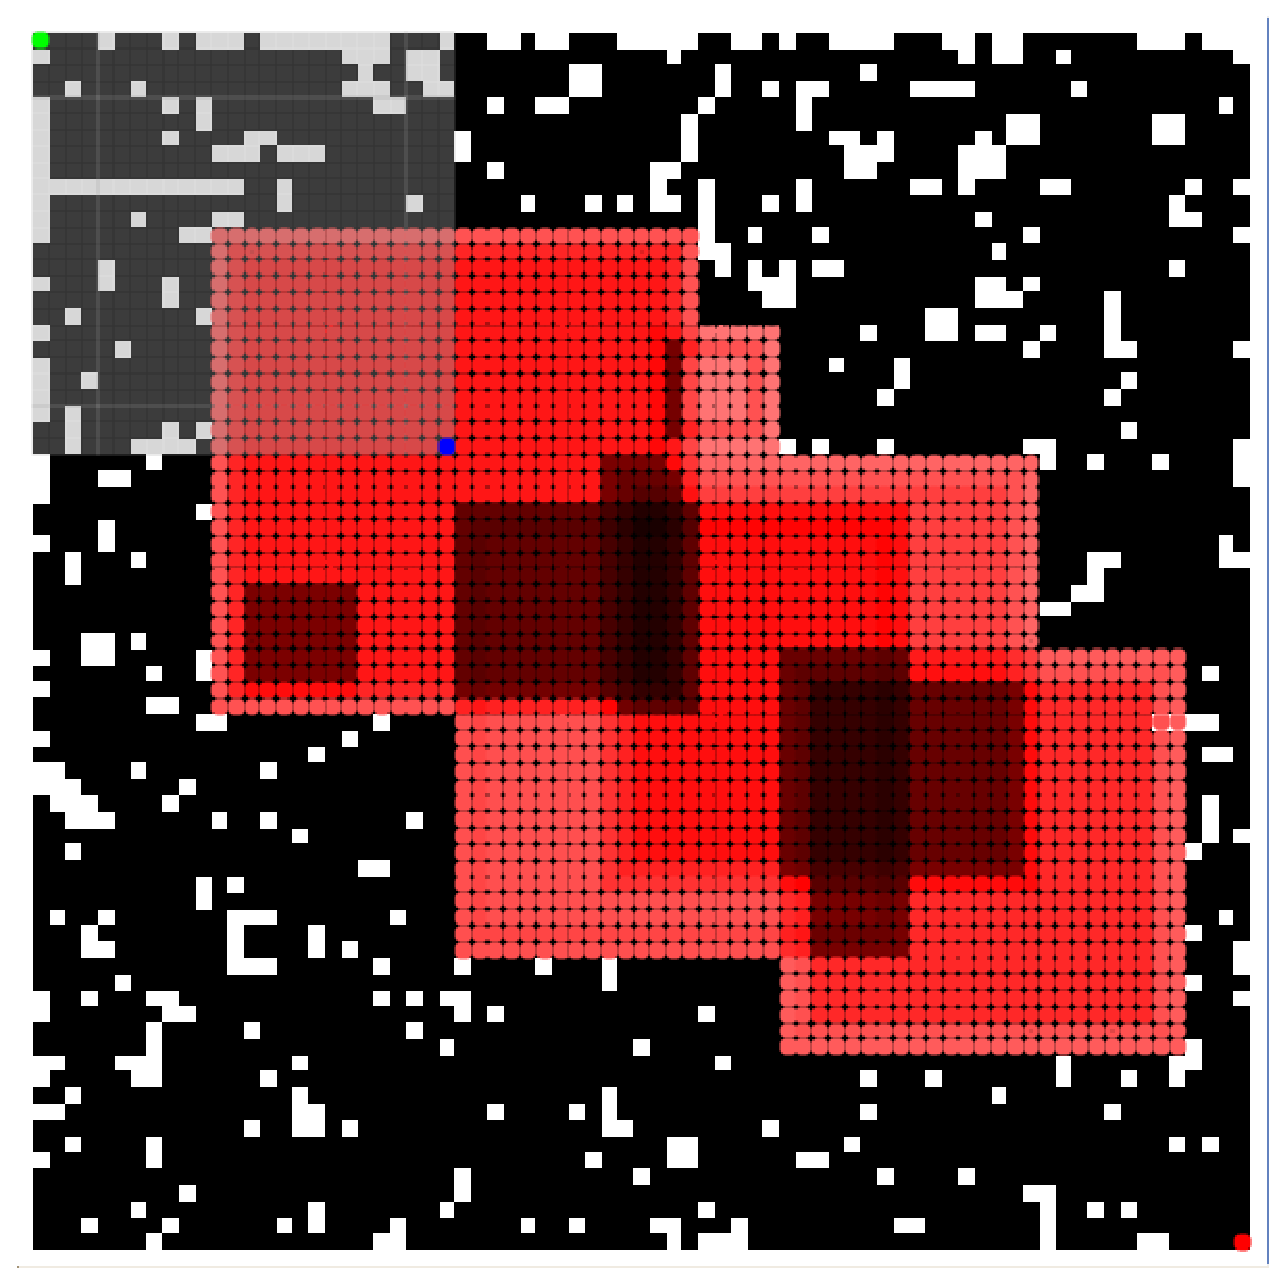
\includegraphics[width=3.5in]{modstarlite/75x75envPropertiesExample}
\caption{A 75 x 75 Visualized Grid Environment}
\label{fig:75x75envExample}
\end{figure}

A simple representation of 2-D grid environment is given in Figure \ref{fig:75x75envExample}. In this figure, white cells are obstacles and black cells are available ones. Agent can traverse all cells except for white ones. The UAV agent is initially placed on upper leftmost cell and painted as green. The target locates on the bottom rightmost and marked as dark red color. The lighter-red square areas represent threat zones. As two threat zones overlaps, the overlapped area becomes darker to represent that risk is increased exponentially on this area. The fogged gray area around UAV agent represents agent's vision range. As agent moves, this area is updated. Thus, agent always chooses the best available cell within her vision range with respect to actual target. This temporary target is marked with blue.

\subsection{The Components and Variables}
MOD* Lite is the multi-objective extension of D* Lite. It can be applied to any unknown dynamic multi-objective search problem where costs can change by time. Considering formal definition; $S$ denotes the set of states in search problem. $s_{start} \in S$ and $s_{goal} \in S$ are the initial and final (target) states, respectively. $pred(s) \subseteq S$ and $succ(s) \subseteq S$ can be used to find predecessors and successors of given state, $s$. The heuristic function $h(s, s')$ which estimates costs between $s$ and $s'$, cost function $c(s, s')$ which represents the actual cost traversing from $s$ to $s'$, actual cost function $g(s)$ and the $rhs(s)$, one-step-lookahead values of $g(s)$ functions are all inherited from D* Lite. However, as we have to consider more than one objective, these functions are to return vector values of scalars instead of scalars. Thus, $rhs(s)$ satisfies the condition

\[ rhs(s) = \left\{ \begin{array}{cc}
ObjectiveVector.MIN & \mbox{if $s=s_{start}$};\\
nonDom_{s' \in pred(s)}(sum(g(s'), c(s', s))) & \mbox{otherwise}.\end{array} \right. \] 

where ObjectiveVector.MIN stands for a vector with $n$ minimum values for an $n$ dimensional problem. These values could be $0$ or $\infty$ for minimization or maximization of objective, respectively. $sum()$ function implements vector summation and $nonDom()$ function returns the set of best non-dominated vectors corresponding to predecessors of any state $s$. Note that $nonDom()$ constructs a list of objective vectors, $rhs(s)$ and $g(s)$ function values are represented as a \textit{lists of objective vectors} where each objective vector in this list is non-dominated with others. An objective vector is a structure that holds values for each objective defined by problem (minimization or maximization). In case of having more than one objective, it is possible that there are more than one paths to a particular state that do not dominate each other. That's why each state might be represented by several vectors. In case we need to compare if one state is better than another, two sets of their vectors need to be compared as formulated below.

\begin{definition}
It can be said that $u$ \textit{completely dominates} $v$ iff $\forall x\in u$ and $\forall y\in v$; $x$ dominates $y$.
\end{definition}

Assume that $\upsilon_{1}=\{[2,5],[3,4]\}, \upsilon_{2}=\{[6,1],[5,2]\}, \upsilon_{3}=\{[3,5]\}$ are lists of objective vectors for three states. $\upsilon_{1}$ and $\upsilon_{2}$ are non-dominated whereas $\upsilon_{1}$ completely dominates $\upsilon_{3}$. 

It could be frankly said that the terms "greater than", "smaller than" and "equals" for scalar value comparison are replaced by "completely dominates", "completely dominated by" and "multi-objectively equals" for vectors of scalars. Non-domination is introduced and handled as the fourth case.

D* Lite introduces local consistency and inconsistency concepts with respect to comparing $g(s)$ and $rhs(s)$. A state is called {\it locally consistent} when $g(s)$ and $rhs(s)$ are equal, and {\it locally inconsistent} otherwise. A locally inconsistent state is referred as locally underconsistent if $g(s)<rhs(s)$ or locally overconsistent if $g(s)>rhs(s)$. In the case of non-domination of these functions, we introduce the concept of {\it local non-consistency}:

\begin{definition}
A state is referred as \textit{locally non-consistent} if its $g(s)$ and $rhs(s)$ values are non-dominated to each other. This inconsistency condition causes the state to reside on more than one solution because it can be understood that two or more predecessors of $s$ are non-dominated to each other.
\end{definition}

Other multi-objective operations are introduced in following subsections. The overall flow of MOD* Lite is given in Algorithm \ref{algMain}.

%% The main algorithm.
\begin{algorithm}
	\caption{Main loop of MOD* Lite}
	\label{algMain}
	%\begin{spacing}{0.5}
	{\fontsize{9}{9}\selectfont
    \begin{algorithmic}[1] % line numbering every line
      \Function{calculateKey}{s}
      	\State $k_{2}$(s)= nonDom(g(s), rhs(s))
      	\State $k_{1}$(s) = sum(h($s_{start}$, s), $k_{m}$, $k_{2}$(s))
      	\State \Return $[k_{1}(s), k_{2}(s)]$
      \EndFunction
   	  \Statex
      \Function{initialize()}{}
      	\State $U = \varnothing $
      	\State $k_{m}$ = ObjectiveVector.MIN
      	\ForAll{$s \in S$}
     		\State rhs(s)=g(s)=ObjectiveVector.MAX
     	\EndFor
      	\State rhs($s_{goal}$) = ObjectiveVector.MIN
      	\State U.insert($s_{goal}$, calculateKey($s_{goal}$))
	  \EndFunction
	  \Statex
	  \Function{plan()}{}
      	\State initialize()
      	\State computeMOPaths()
      	\While{$true$}
    	      	\State solutionPaths = generateMOPaths()
    	      	\If{solutionPaths = null} there is no known path \EndIf
    	      	\State Wait for any weight cost to change;
    	      	\If{Any weight cost changes}
    	      		\State $k_{m}$ = sum($k_{m}$, h($s_{goal}$, $s_{start}$))
    	      		\ForAll {Changed weight costs of edges(u,v)}
    	      			\State Update cost c(u,v)
    	      			\State updateVertex(u)
    	      		\EndFor
		      	\State computeMOPaths()
    	      	\EndIf
		\EndWhile
  	  \EndFunction
    \end{algorithmic}}
    %\end{spacing}
\end{algorithm}

Basically, D* Lite tries to make all states locally consistent. Locally inconsistent states are maintained in  a priority queue (U) with their key values and expanded considering priority values. However, locally non-consistent states cannot be maintained in such a queue due to the non-domination of their key values, which are also set of objective vectors. If two keys cannot be dominated by each other, they should be criticized in the same manner. Thus, a more convenient structure; a directed acyclic state expansion graph instead of a priority queue which uses topological ordering of states with respect to the key domination, is presented. In this model, the graph (U) contains set of nodes each represented by a state and its key value. When a state is to be added into U with $insert(state, key)$ operation, key value is compared with all existing nodes' key values. If the new state dominates some state, an edge is introduced from the new state to this state. No edge connection is done in case of multi objectively equality and non-domination. As a result, incoming and outgoing degrees of a node $s$ correspond to the number of nodes that \textit{dominates} $s$ and the number of nodes that are \textit{dominated by} $s$, respectively. The node(s) with incoming degree 0 are the non-dominated nodes where none of other nodes could dominate. $topKey()$ and $topKeys()$ return the key value(s) of nodes with minimum incoming degree. $pop()$ returns and removes the state (all its incident -incoming and outgoing- edges are also removed from the graph) with minimum incoming degree. Another strategy for $pop()$ operation could be removing the state with maximum outgoing degrees where the number of outgoing degree of a state $s$ presents that how many states are dominated by $s$. Also, these two methods could be combined where two topologically ordered lists, one is for minimum incoming degrees and the other is for maximum outgoing degrees, are maintained and a state which has both minimum incoming and maximum outgoing degrees according to these lists could be selected. As these strategies could be set to applied domain according to its requirements, we choose selecting and removing from minimum incoming degrees list. If more than one nodes exist with minimum degree, one of them is selected randomly. $remove(state)$ operation removes a given state and its incident edges from graph. An example of a state expansion graph with states and their corresponding key values is given in Figure \ref{fig:graph1}. Incoming degrees of nodes are given as a list in the figure.

\begin{figure}
\centering
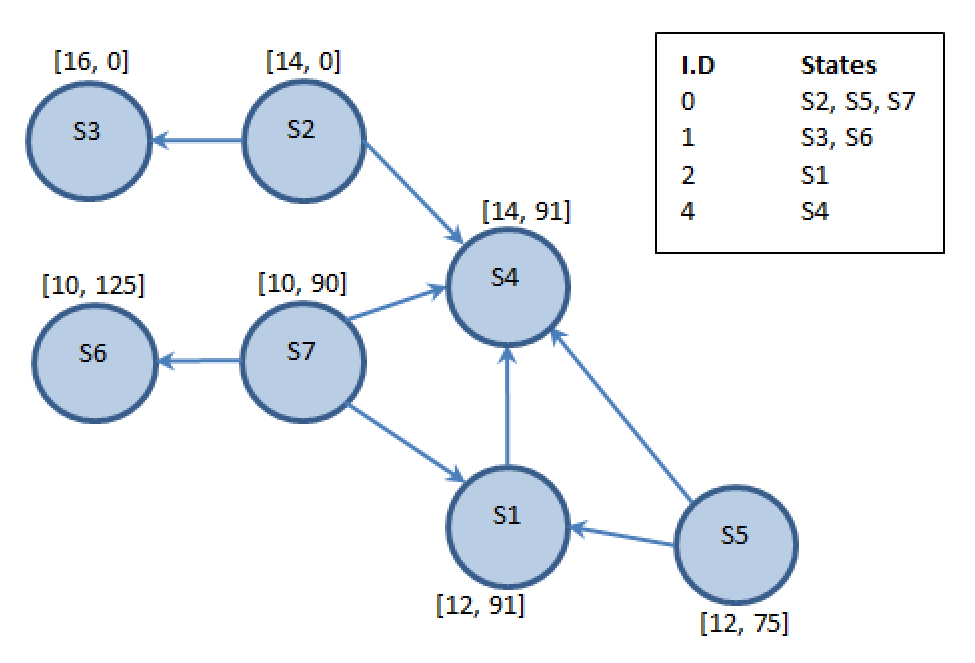
\includegraphics[width=2.5in]{modstarlite/graph1v2}
\caption{Directed Acyclic State Expansion Graph}
\label{fig:graph1}
\end{figure}

Addition of a new state to the state expansion graph is illustrated in Figure \ref{fig:graph2}.  $S8$ is  "the new" state to be added, the dashed directed edges are established between $S8-S1$, $S8-S4$ and $S8-S5$ because $S8$'s key can only dominate keys of nodes $S1, S4$ and $S5$. None of the existing states' keys can dominate $S8$, so incoming degree of $S8$ becomes 0. This addition also effects the incoming degrees list where the changed positions are highlighted in the figure. Addition of $S8$ increments the incoming degrees of $S1$, $S4$ and $S5$ by 1 so their positions are shifted down.

\begin{figure}
\centering
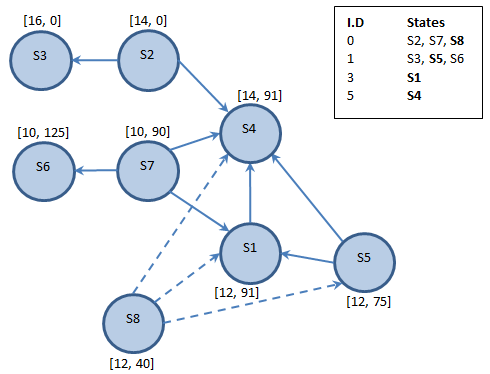
\includegraphics[width=2.5in]{modstarlite/graph2v2}
\caption{State Expansion Graph after Adding State $S8$}
\label{fig:graph2}
\end{figure}

\subsection{Key Formulation}
In the previous subsection, it is stated that the directed acyclic graph structure is used to determine expansion of nodes in state space with their \textit{keys}. The basic idea behind the calculation of keys is similar with D* Lite, with slight modifications. As MOD* Lite is considered in a multi-objective setting, key value is stated as a vector with two components: $k(s) = [k_{1}(s);k_{2}(s)]$ where these components are set of objective vectors. $k_{2}(s)$ is calculated by finding the \textit{non-dominated list} of $g(s)$ and $rhs(s)$, where $k_{2}(s)= nonDom(g(s), rhs(s))$. The other component, $k_{1}(s)$  is calculated as vector summation of $h(s_{start}, s), k_{m}$ and $k_{2}(s)$. Calculation of $k(s)$ can be seen in lines \{2 and 3\} in Algorithm \ref{algMain}. $k_{m}$ is used for heap reordering as defined in  D* Lite.

\begin{algorithm}
	\caption{Update Vertex \& Compute Multi-Objective Paths}
	\label{algUpdate}
    \begin{algorithmic}[1]
   	  \Function{updateVertex}{u}
   	  	\If{$u \neq s_{goal}$}
   	  		\State $rhs(u) = nonDom_{s' \in succ(u)}(sum(c(u,s'), g(s')))$
   	  	\EndIf
   	  	\If{$u \in U$} U.remove(u) \EndIf
   	  	\If{!equals(g(u), rhs(u))}
   	  		\State U.insert(u, calculateKey(u))
   	  	\EndIf
   	  \EndFunction
    	  \Statex
      \Function{computeMOPaths()}{}
		\While{dominatesAll(calculateKey($s_{start}$), U.topKeys())}
		% OR !equals(rhs(s_{start}, g(s_{start}))$}
			\State $k_{old}$ = U.topKey()
	      	\State u = U.pop()
	      	\State $k_{new}$ = calculateKey(u)
	      	\If{$k_{old}$.completelyDominates($k_{new}$) }
	      		\State U.insert(u, $k_{new}$)
	      	\ElsIf{rhs(u).completelyDominates(g(u))}
	      		\State g(u) = rhs(u)
	      		\ForAll{$s \in pred(u)$} $updateVertex(s)$ \EndFor
	      	\ElsIf{g(u).completelyDominates(rhs(u))}
	      		\State g(u) = ObjectiveVector.MAX
	      		\ForAll{$s \in pred(u) \cup \{u\}$} $updateVertex(s)$ \EndFor
	      	\Else
	      		\State g(u) = nonDom(g(u), rhs(u))
	      		\ForAll{$s \in pred(u)$} $updateVertex(s)$ \EndFor
	      	\EndIf
		\EndWhile
	  \EndFunction
	\end{algorithmic}
\end{algorithm}

\subsection{Details of MOD* Lite}
MOD* Lite is based on  D* Lite algorithm as introduced in the previous section. There are fundamental differences due to the structures used and the way the solution paths are maintained. The pseudocode of MOD* Lite is given in Algorithms \ref{algMain}, \ref{algUpdate} and \ref{algPathGen}.

First of all, searching order of MOD* Lite is from goal to start state, like D* Lite. The main function of MOD* Lite first calls $initialize()$ to set up the execution in Algorithm \ref{algMain}. This function calculates the key value for goal state, adds it into U and sets the rhs value to a \textit{MIN} objective vector, which has minimized n values for n-objectives. These values can be $0$ for minimized-objective and $\infty$ for maximized-objective. Then, proper $g(s)$ values are calculated considering all objectives with $computeMOPaths()$. Finally, paths are generated with these $g(s)$ values. If a weight cost is changed in the environment, corresponding states are re-expanded and only related weights are updated. Notice that this cost change might happen for only one objective or several objectives at the same time.

The $computeMOPaths()$ pseudocode is given in Algorithm \ref{algUpdate} line \{7\}. The termination criteria of this function is where the key of $s_{start}$ dominates all the top keys returned from U. Until it terminates, the top state is sequentially selected from top states of U and expanded. While expanding a state, the domination between g and rhs values of corresponding state is observed. If $rhs(s)$ values completely dominate $g(s)$ values, local underconsistency case occurs. We apply the same strategy with D* Lite, update g value with rhs and update weights for all predecessors of s with $updateVertex()$. If $g(s)$ values completely dominate $rhs(s)$ values, the case is locally overconsistency. Simply g value for this state is set as \textit{MAX} objective vector, which is $\infty$ for minimized-objective and $0$ for maximized one, and current state weight is updated with its predecessors' weight. The third case occurs when g and rhs values can not completely dominate each other, \textit{locally non-consistency}. In this case, g value is updated with non-dominated values of g and rhs values and again predecessors of current state is updated. Keeping non-dominated values of g and rhs enables to keep track of each non-dominated successors' information.

To update a weight of a state, MOD* Lite uses $updateVertex(u)$ shown in Algorithm \ref{algUpdate} line \{1-6\}. It simply adds corresponding state to or removes from U according to given criteria. While updating $rhs(u)$ except goal state, non-dominated objective values of multi-objectively summed $c(u,s')$ and $g(s')$ are established and used.

After state expansion operation is finalized and corresponding $g(s)$ values are set, multi-objective paths are generated via these $g(s)$ values by given pseudocode in Algorithm \ref{algPathGen}. Path generation is achieved in two phases: setting parent(s) for each non-dominated successor of expanding state and constructing paths by following (backtracking) these parents. The first phase is performed from the start to the goal state whereas the second is from the goal to the start state. 

A queue is used to keep track of expanding states which is shown in line \{2\}. This queue initially has $s_{start}$ only. Thus, starting from $s_{start}$, the while loop iterates until this queue becomes empty. Finding a goal state is not considered as a termination criteria because other non-dominant paths might be available. As expanding a state, we refer to set \textit{it} as a parent to its successors indicated between lines \{7-36\}.

Before expansion of a state $s$, non-dominated successors are found first with respect to multi-objective summation of $c(s,s')$ and $g(s')$ as shown in line \{5\}. If a successor $s'$ is found in non-dominated successors list, it has a potential to have $s$ as a parent. For each non-dominated successor $s'$, first parents list of $s$ is checked. If $s$ does not have any parent, which only occurs iff $s=s_{start}$, for sure $s'$ does not have any parent as well. In this case, $s$ is added  as a parent of $s'$ with corresponding cost $c(s,s')$. Parents of a state are kept in a map where keys of this map are parents and values are cumulative costs which is consumed to reach that state from start through corresponding parent. These costs are used to determine elimination of existing parents when a new one is considered to be added. This idea will be elaborated later.

% Indentations are used make visualization better.
\begin{algorithm}
	\caption{Path Generator Algorithm}
	\label{algPathGen}
    \begin{algorithmic}[1]
    		\Function{generateMOPaths()}{}
			\State expandingStates.add($s_{start}$)
    			\While{!expandingStates.isEmpty()}
    				\State s = expandingStates.poll()
				\State nonDomSuccs = $nonDom_{s' \in succ(s)}$(sum(c(s, s'), g(s'))
    				\ForAll{$s'\in nonDomSuccs$}
    					\If{s.parents() = null}
    						\State s'.parents().put(s, c(s, s'))
    					\Else
    						\State cumulativeC = sum(c(s, s'), s.parents().values())
    						\If{s'.parents() = null}
    							\State s'.parents().put(s, cumulativeC)
    						\Else
							\ForAll {$s'' \in s'.parents()$}
								\If{equals(s'.parents(s''), cumulativeC) OR completelyDominates( s'.parents(s''), cumulativeC)}
									\State \textbf{break}
								\ElsIf{completelyDominates(cumulativeC, s'.parents(s''))}
									\State s'.parents().remove(s'')
									\State s'.parents().put(s, cumulativeC)
								\Else
									\ForAll{$cC \in cumulativeC$}
										\ForAll{$eC \in s'.parents(s'')$}
											\If{eC.equals(cC) OR eC.dominates(cC)}
												\State cumulativeC.remove(cC) 
												\State \textbf{break}
											\ElsIf{cC.dominates(eC)}
												\State s'.parents(s'').remove(eC) 
												\State \textbf{break}
											\EndIf
										\EndFor
										\If{s'.parents(s'') = null}
											\State s'.parents().remove(s'')
										\EndIf
									\EndFor
									\If{!cumulativeC = null}
											\State s'.parents().put(s, cumulativeC)
									\EndIf
								\EndIf
							\EndFor    						
    						\EndIf
    					\EndIf
    					\If {s'.parents.contains(s) AND !expandingStates.contains(s')}
    						\State expandingStates.add(s')
    					\EndIf
    				\EndFor
    			\EndWhile
    			\State solutionPaths = construct paths recursively traversing parents
    			\State \Return solutionPaths
    		\EndFunction
	\end{algorithmic}
\end{algorithm}

If $s$ has predefined parents (starting from \{9\}), a cumulative total cost is calculated for $s'$ in line \{10\}. This cost is multi-objective summation of $c(s, s')$ and aggregated cost values of parents of $s$. Notice that the algorithm proves that parents' costs of a state are always non-dominated to each other, so the aggregated cost values contain \textit{all} parents' \textit{all} costs. These cost values express all non-dominated solution costs to reach that state. If $s'$ does not have any parent up to now (\{11\}), $s$ is added as a parent of $s'$ with cumulative cost. Else, each existing parent of $s'$, say $s''$ should be compared with the cumulative cost. These operations are shown in lines between \{13-32\}. Here, if $s''$ has same cost with or better cost (determined by completely domination term) than cumulative cost, needless to say that $s$ is not required to be added as a parent to $s'$. Otherwise, if cumulative cost completely dominates $s''$, it can be inferred that one can reach $s'$ from $s$ in a better way than $s''$. Thus, $s''$ is removed from parents of $s'$ and $s$ is added with the cumulative cost. The fourth possibility occurs when costs of $s''$ and cumulative costs do not completely dominate each other. In this situation, each cost in cumulative costs is compared with each cost of $s''$ costs. Equality or domination probabilities causes to remove corresponding cost from its list. At the end of the comparison, $s''$ is removed from parents of $s'$ if all of its costs are dominated (lines \{29-30\}) and $s$ is added as a parent if cumulative costs still have non-dominated cost (lines \{31-32\}).

After organizing parents of $s'$, it is decided to expand it in following iterations. If $s$ is successfully added as a parent and expanding states queue does not already have it, $s'$ is added to the tail of the queue. This can be seen in lines \{33-34\}.

When all non-dominated parents are properly set from start to goal state, these parents can be followed recursively starting from goal towards start state and multi-objective paths are constructed. Finally, all found paths have non-dominated path costs regarding to each other.

\section{A Multi Objective Genetic Path Planner : MOGPP}

Many real-life optimization problems are NP-hard where optimal solutions could not be found in polynomial time. As evolutionary computing methods are classified as stochastic soft-computing methods and can be applied to NP-hard problems, several genetic algorithms are developed with respect to this problem \cite{Pangilinan}, \cite{Peng_Xu_Zhang:2011}. To show that MOD* Lite gives feasible and qualified solutions, it is a must to compare it with a stochastic evolutionary method. Thus, a multi objective genetic path planner, MOGPP is also developed in the scope of this study.

\subsection{Overview}

Multi objective genetic path planner (MOGPP) proposed in this study is an alternative solution for finding paths on virtual environments considering multiple objectives. It proposes a classical genetic algorithm structure with crossover and mutation operations where each individual represents a valid path from initial location to target. Experimental and performance results show that MOGPP finds paths in exponential times with respect to MOD* Lite, which are detailed in next section. The chromosome structure, fitness function, crossover, mutation and details of the MOGPP are given in following subsections.

\subsection{Chromosome Representation}

Like all evolutionary algorithms, MOGPP come up with a population where each individual of the population is represented by a chromosome structure. This structure simply stands for a valid path from initial location to target, a legal solution for the problem. Thus, each gene in chromosome is a \textit{cell} in this valid path. As the solution path' s lengths differ from each other, the chromosome lengths may diversify.

\subsection{Fitness Function}

The fitness function is crucial to evaluate a chromosome which is tested for suitability for the environment under some consideration. As the genetic algorithm proceeds, it is expected that the fitness value of the "best" chromosome increases as well as the total fitness of the population as a whole.

The fitness function used in MOGPP is given as follows; \[F(i) = [\dfrac{1}{pathLength(i)^{2}}], [\dfrac{1}{exposuredRisk(i)^{2}}] \] which is the fitness function of individual $i$ in population. This function is represented by a vector of objectives, where first objective is inverse of path length square of corresponding individual and second objective is inverse of calculated exposured risk square during this path. The purpose of fitness function is to yield better results when an individual's path is shorter and safer. On the evaluation process, these fitness values of all individuals in the population are added multi objectively and evaluation value is calculated. The evolution of population is determined by this total fitness value.

\subsection{Crossover Operation}

In genetic algorithms, crossover operation is used to vary the chromosomes and generate new individuals from existing ones. But, to breed new individuals and to use the operators borrowed from natural genetics, the parents should be selected first. There exists many selection operations for genetic algorithms. For MOGPP, roulette-wheel selection method is used to keep the algorithm simple. With this way, greater fitness evaluation owner chromosomes have bigger opportunity to be selected. This mechanism facilitates the population to evolve.

As a single chromosome stands for a valid path in MOGPP, new generated children should also obey this rule. Thus, genetic operations must guarantee that new generated children are consistent and have valid paths. For crossover operation used in MOGPP, assume that two parents' paths are represented by 
\begin{gather*}
P(i)=\lbrace \varsigma, ..., c_{i-1}, c_{i}, c_{i+1}, ..., \tau \rbrace \\
P(j)=\lbrace \varsigma, ..., c_{j-1}, c_{j}, c_{j+1}, ..., \tau \rbrace
\end{gather*}
for $i$ and $j$ individuals. $\varsigma$ and $\tau$ shows initial and target locations, respectively. While crossover, an intersected cell of these paths is determined. Then, each path is split up into two sub-paths referencing by this cell. If this cell is $c_{i} = c_{j}$, the splitting operation is done as follows
\begin{gather*}
P(i)_{1}=\lbrace \varsigma, ..., c_{i-1} \rbrace \\
P(i)_{2}=\lbrace c_{i}, c_{i+1}, ..., \tau \rbrace \\
P(j)_{1}=\lbrace \varsigma, ..., c_{j-1} \rbrace \\
P(j)_{2}=\lbrace c_{j}, c_{j+1}, ..., \tau \rbrace
\end{gather*}
The concatenation of swapped sub-paths generate new individuals
\begin{gather*}
P'(i)=\lbrace P(i)_{1}, P(j)_{2} \rbrace \\
P'(j)=\lbrace P(j)_{1}, P(i)_{2} \rbrace 
\end{gather*}
$P'(i)$ and $P'(j)$ are the new crossovered paths for parents $i$ and $j$. Also, visualized representation of crossover operation is given in Figure \ref{fig:xover}.

\begin{figure}
\centering
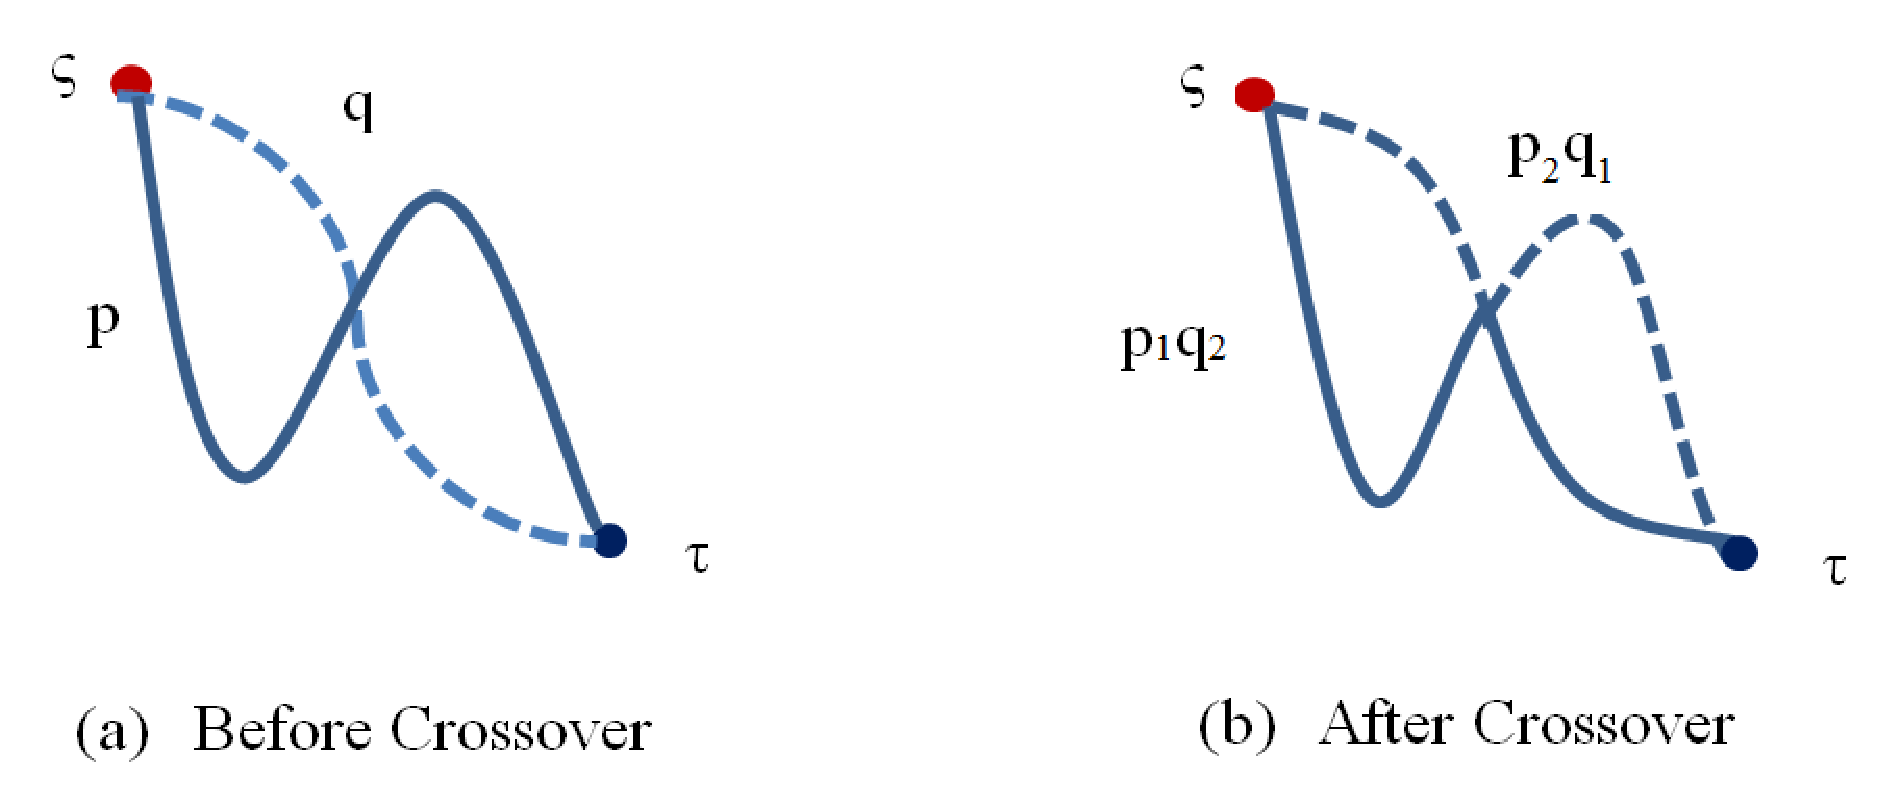
\includegraphics[width=2.5in]{mogpp/xover}
\caption{Crossover Operation}
\label{fig:xover}
\end{figure}

\subsection{Mutation Operation}

In genetic algorithms, mutation is used to maintain genetic diversity of the population. In MOGPP, with respect to given chromosome structure; a cell from corresponding individual' s path is selected randomly first. This cell is the reference point to split up the path into two sub-paths. Then, the sub-path which contains target location is thrown away and a random path to the target is generated instead. The visualization of mutation is given in Figure \ref{fig:mutation}.

\begin{figure}
\centering
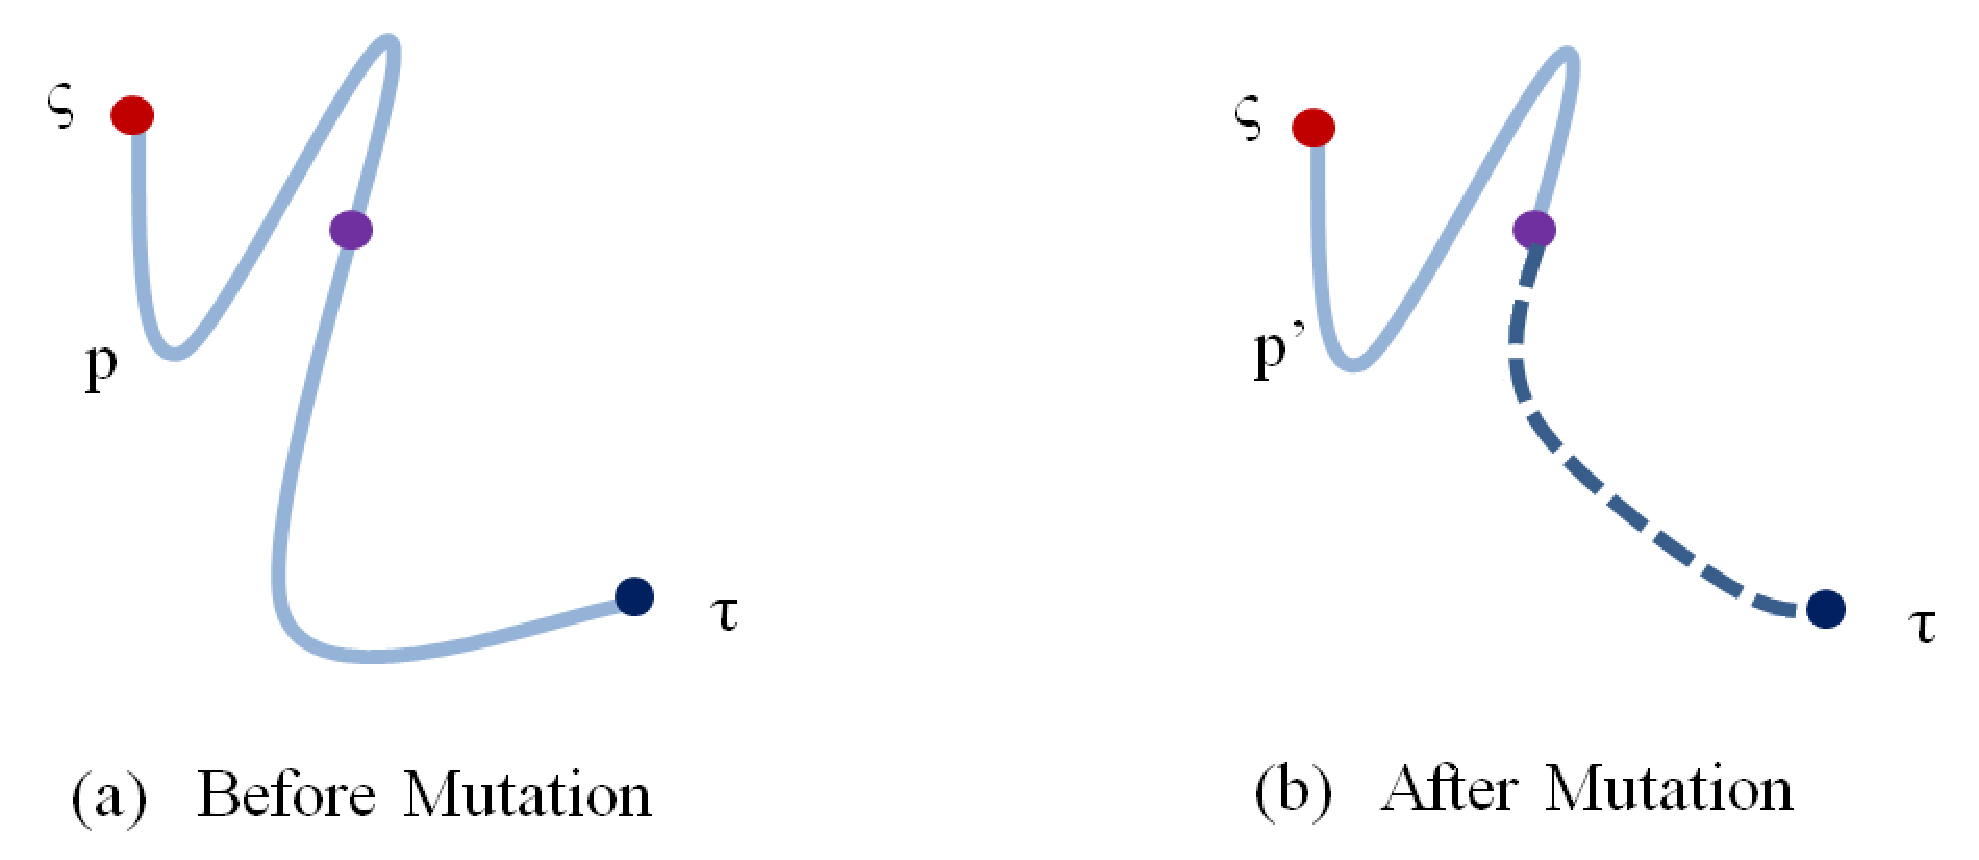
\includegraphics[width=2.5in]{mogpp/newMutation}
\caption{Mutation Operation}
\label{fig:mutation}
\end{figure}

\subsection{Details of Algorithm}

As mentioned above, MOGPP is designed based on a simple classic genetic algorithm structure. Main loop of MOGPP is given in Algorithm \ref{algMOGPP}.

\begin{algorithm}
	\caption{MOGPP : Main Loop}
	\label{algMOGPP}
    \begin{algorithmic}[1]
    	  \Function{evolve()}{P}
	  	\State $P' = \varnothing$
	  	\State $P'.addAll(elites(P))$
	  	\While{$P'.size < P.size$}
	  		\State $parents = selectParents(P)$
	  		\State $crossover(parents)$
	  		\State $mutate(parents)$
		  	\State $P'.addAll(parents)$
	  	\EndWhile
	  	\State \Return $P'$
      \EndFunction
   	  \Statex
      \Function{initializePopulation()}{}
      	\State $P = \varnothing$
      	\For{$i = 1 \to POPULATION\_SIZE$}
      		\State $P(i) = generateRandomPath(\varsigma, \tau)$
      	\EndFor
      	\State $evaluate(P)$
		\State \Return $P$
	  \EndFunction
	  \Statex
	  \Function{plan()}{}
      	\State $P = initializePopulation()$
      	\While{$reached\ to\ MAX\_ITERATION$}
    	      	\State $P = evolve(P)$
    	      	\State $evaluate(P)$
		\EndWhile
		\State \Return $bestIndividuals(P)$
  	  \EndFunction
	\end{algorithmic}
\end{algorithm}

Initialization of algorithm starts with $plan()$ function. At first, random valid paths from initial location ($\varsigma$) to the target ($\tau$) are generated. Notice that these paths do not contain any ties, to simplify and speed up genetic operators' processes.

Each generated path represents an individual in population. These individuals are kept in a directed acyclic graph to cope with multi objectivity. The vertices and edges represent individuals and domination of multi objective path costs of these individuals, respectively. If a path cost of an individual dominates to other's, an edge is established between these individuals' vertices. Non domination and equality do not come up with an edge. When an individual is generated and desired to be added to population, the cost function of this individual is compared with existing individuals' costs and required edge connections are established. The directed acyclic graph structure has the same essence and representation with MOD* Lite' s priority structure, which was detailed in previous section. 

After population initialization, all individuals are evaluated with respect to their fitness functions. The evaluation gives better results when an individual's path is shorter and safer. Total fitness value is calculated by adding all individuals' fitness values multi objectively. This value increases while population is evolving.

The evolution process is applied to all individuals of a population. When a population is evolving, predefined number of best individuals are transferred to new population first. Then, two individuals are selected as parents by roulette wheel selection method. This method gives higher chances to the individuals which have better fitness functions to be selected. After two parents are selected, crossover and mutation is applied with predefined distinct probabilities.

After a predefined number of iterations (the maximum iteration count), algorithm is halted and elite individuals are taken as multi objectively best results.

Notice that the amount of initially generated individuals - population size -, maximum iteration count of evolution, number of elite individuals selected on each evolution phase, crossover and mutation probabilities should be predefined and set before the execution of MOGPP.
